\section{Method}
\label{sec:method}

\subsection{System Architecture}
\label{subsec:method-architecture}

GaitNet is the contact-selection layer of a hierarchical stack
(\autoref{fig:architecture}). A terrain map is converted into a
per-leg validity mask. GaitNet scores every valid cell together with a
learned no-action option and issues at most one footstep command. The
execution controller turns that command into a contact schedule, a
swing trajectory, and joint torques. \autoref{tab:stack} lists the
components used at each stage. The same policy weights are used in
all stages; they are frozen after training and are not fine-tuned.

\begin{table}[t]
  \centering
  \caption{Components used at each stage.}
  \label{tab:stack}
  \footnotesize
  \setlength{\tabcolsep}{2.5pt}
  \newcolumntype{L}[1]{>{\raggedright\arraybackslash}p{#1}}
  \begin{tabular}{@{}L{0.17\linewidth}L{0.26\linewidth}L{0.26\linewidth}L{0.26\linewidth}@{}}
    \toprule
    & \textbf{Training} & \textbf{Evaluation} & \textbf{Hardware} \\
    \midrule
    Platform & Isaac Lab \cite{mittal_orbit_2023}, $\Delta t{=}\corlPhysicsDtMs$\,ms
      & Gazebo (ODE), $\Delta t{=}\corlGazeboStepMs$\,ms & Unitree Go1 \\
    Controller & Convex MPC \cite{di_mini_cheetah_2020,
      zhuang_rl_mpc_locomotion_2025}, \corlTrainMpcHz\,Hz
      & NMPC/WBC \cite{leggedcontrol, leggedperceptive}
      & NMPC/WBC \cite{leggedcontrol, leggedperceptive} \\
    NMPC / WBC rate & -- & \corlNmpcHz\,Hz / \verify{XX}\,Hz
      & \corlNmpcHz\,Hz / \corlWbcHz\,Hz \\
    Terrain source & Ray-cast height field & Simulated depth camera
      $\rightarrow$ elevation map & Intel D435i $\rightarrow$
      elevation map \\
    Planner rate & \corlControlHz\,Hz & \pending{\corlControlHz\,Hz}
      & $\le$\,4\,Hz (\autoref{subsec:exp-hardware}) \\
    Policy weights & Trained & Frozen & Frozen \\
    \bottomrule
  \end{tabular}
\end{table}

\begin{figure*}[t]
  \centering
  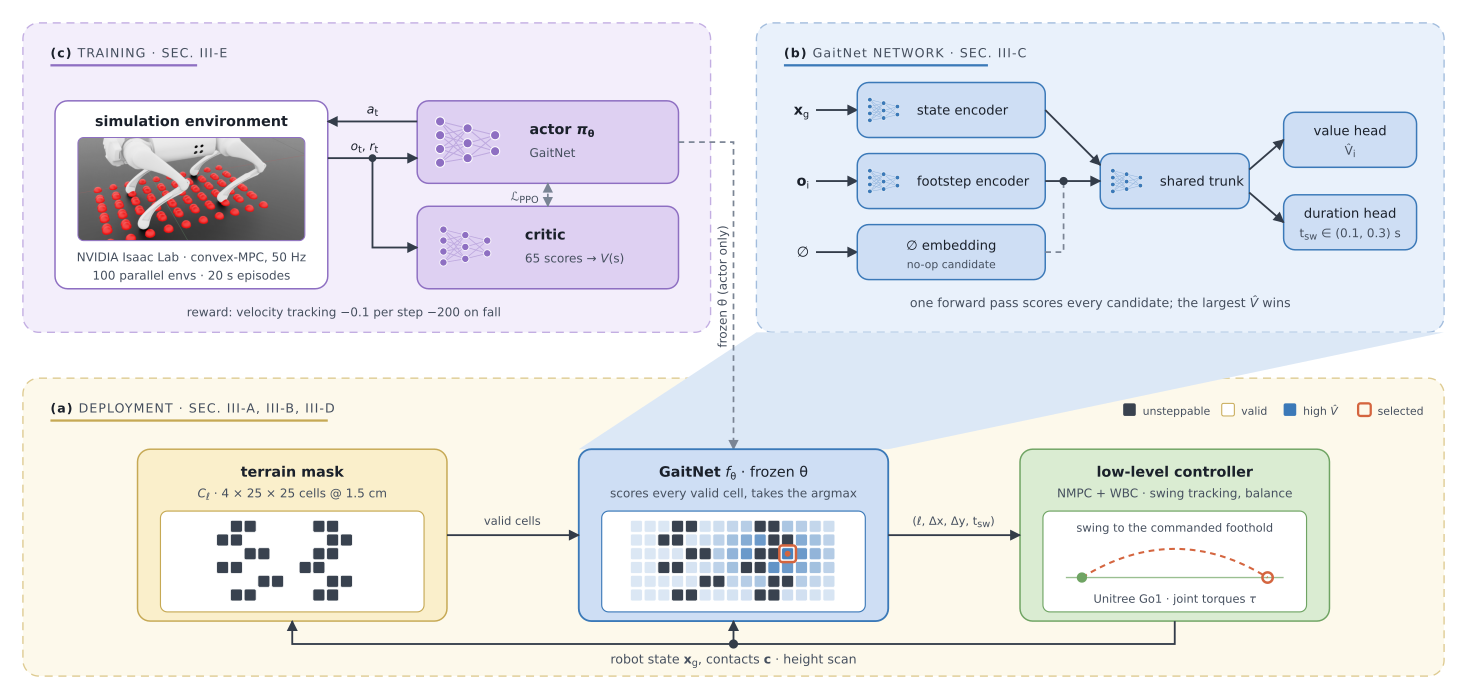
\includegraphics[width=\textwidth]{images/diagrams/gaitnet-architecture.png}
  \caption{System overview. (a)~Deployment: an elevation map becomes a
    per-leg validity mask; GaitNet scores every valid cell plus a
    no-action option in one batched pass, and the argmax is issued as a
    single footstep command to the execution controller. (b)~Network:
    state and candidate embeddings feed a shared trunk with value and
    duration heads. (c)~Training: PPO in Isaac Lab over a sampled
    \corlTrainTotalCandidates-candidate set; only the actor is
    deployed.}
  \label{fig:architecture}
\end{figure*}

In both Gazebo and on the Go1, execution uses the
\texttt{legged\_control} NMPC/WBC framework \cite{leggedcontrol} with
its perceptive extension \cite{leggedperceptive}, built on OCS2. The
NMPC is solved with SQP at \corlNmpcHz\,Hz over a
\corlNmpcHorizon\,s horizon, and a weighted WBC computes joint
torques. The native gait scheduler is replaced by GaitNet commands;
the NMPC, WBC, state estimator, and terrain pipeline are unchanged.
The terrain pipeline builds an elevation map
(\corlElevMapSizeM$\times$\corlElevMapSizeM\,m, \corlElevMapResCm\,cm
cells) from a depth point cloud and decomposes it into convex planar
regions. In Gazebo the point cloud comes from a simulated depth camera,
not from ground-truth geometry, so perception error is present in
evaluation.

\subsection{Planner--Controller Interface}
\label{subsec:method-interface}

At decision time $t$, GaitNet implements the map
\begin{equation}
  \mathcal I_t = \left(x_t,\ \mathcal M_t,\ c_t\right)
  \longmapsto
  \left(\ell_t,\ \Delta p_t,\ T^{\mathrm{swing}}_t\right).
  \label{eq:interface}
\end{equation}
The inputs are:
\begin{itemize}
  \item $x_t$: a controller-independent measured robot state
    (\autoref{eq:state});
  \item $\mathcal M_t = \{M^{i}_t\}_{i=1}^{4}$: per-leg Boolean
    validity masks, each a $\corlGridCells\times\corlGridCells$ grid
    with \corlMaskResolutionCm\,cm cells centered on the projection of
    hip $i$ and aligned with the base yaw;
  \item $c_t\in\{0,1\}^{4}$: per-leg contact/swing status.
\end{itemize}
The outputs are:
\begin{itemize}
  \item $\ell_t \in \{\mathrm{FR},\mathrm{FL},\mathrm{RR},\mathrm{RL},
    \varnothing\}$: the selected leg, where $\varnothing$ denotes no
    action;
  \item $\Delta p_t \in \mathbb R^2$: the foothold target as an $xy$
    offset from the selected hip in the yaw-aligned base frame. The
    target height is taken from the terrain map, not from GaitNet;
  \item $T^{\mathrm{swing}}_t$: the requested swing duration.
\end{itemize}

The controller realizes a command as follows. The foothold is anchored
in the odometry (world) frame at commit time, so it does not drift
with the base during the swing. The swing interval is inserted into
the NMPC mode schedule, and the foothold is passed to the
convex-region selector, which projects it onto the best planar region
and constrains the swing target near the projected point. GaitNet
never reads the NMPC cost, constraints, or solution.

This interface assumes an execution controller that
(i)~accepts explicit foothold targets; (ii)~accepts, or can
approximate, the requested swing duration; (iii)~tracks a commanded
base velocity; (iv)~provides estimated body and foot states; and
(v)~provides contact or swing status. GaitNet is decoupled from the
controller's internal formulation, but it is not independent of
controller tracking quality.

\subsection{High-Rate Acyclic Selection}
\label{subsec:method-selection}

GaitNet is trained to decide every \corlControlTickMs\,ms
(\corlControlHz\,Hz). Each decision issues at most one footstep; all
other legs keep their current commands. Because a swing lasts
\corlSwingDurationMin--\corlSwingDurationMax\,s, between
\numberstringnum{\corlMinTicksPerSwing} and
\numberstringnum{\corlMaxTicksPerSwing} decisions occur before the
swinging leg touches down. At each of them GaitNet may commit another
leg. Swing overlap therefore arises from the value function and the
repeated decision rule, not from a configured gait.

Two feasibility rules are applied before scoring. A leg already in
swing is removed from the mask and its target is not redirected. A new
step is permitted only if at least
\numberstringnum{\corlMinContactLegs} legs are in contact, which
bounds concurrency at \numberstringnum{\corlMaxConcurrentSwingLegs}
swinging legs. In training the mask is additionally dilated with
\numberstringnum{\corlMaskDilationRounds} rounds of max pooling to
account for foot size and state-estimation error.

\subsection{Network}
\label{subsec:method-network}

The robot state is
\begin{equation}
  x_t =
  \begin{bmatrix}
    \mathbf p_{f,xy}^{b} &
    p_{b,z}^{w} &
    \mathbf v_b^{b} &
    \boldsymbol\omega_b^{b} &
    \mathbf v^{\mathrm{cmd}} &
    c_t &
    \mathbf g^{b}
  \end{bmatrix}^\top \in \mathbb R^{\corlStateDim},
  \label{eq:state}
\end{equation}
where superscript $b$ denotes the base frame and $w$ the world
(odometry) frame. $\mathbf p_{f,xy}^{b}\in\mathbb R^{\corlFootPosDim}$
holds the $xy$ positions of the four feet, $p_{b,z}^{w}$ is base
height, $\mathbf v_b^{b}$ and $\boldsymbol\omega_b^{b}$ are base linear
and angular velocity, $\mathbf v^{\mathrm{cmd}}=[v_x,v_y,\omega_z]$ is
the commanded base velocity, and $\mathbf g^{b}$ is the unit gravity
vector expressed in the base frame. Using projected gravity avoids a
quaternion input and its ordering convention.

A \numberstringnum{\corlStateEncoderLayers}-layer MLP (hidden size
\corlStateEncoderHidden) encodes $x_t$. A
\numberstringnum{\corlFootstepEncoderLayers}-layer MLP (hidden size
\corlFootstepEncoderHidden) encodes each candidate's leg one-hot and
hip-relative offset; the no-action option uses a separate learned
embedding. The two embeddings are concatenated
\cite{feng2021deep} and passed through a
\numberstringnum{\corlTrunkLayers}-layer trunk with two heads. The
value head outputs an unnormalized logit $\hat V$ used for ranking,
and the duration head outputs $T^{\mathrm{swing}}$, mapped by a sigmoid
into $(\corlSwingDurationMin,\corlSwingDurationMax)$\,s. All
activations are ReLU.

\subsection{Candidate Enumeration}
\label{subsec:method-enumeration}

At deployment, GaitNet enumerates every mask cell rather than sampling.
Each leg's grid spans $\pm\corlGridReachCm$\,cm around the hip, giving
$\corlNumLegs\times\corlCellsPerLeg=\corlSpatialCandidates$ footholds
plus no-action, i.e.\ \corlTotalCandidatesDense{} candidates. Invalid
cells are discarded before scoring.

Enumeration is cheap because the candidate embedding does not depend
on the state. The embeddings of all grid cells are computed once and
cached, so each decision requires one state-encoder pass and one
batched trunk pass. In an isolated process, scoring all
\corlTotalCandidatesDense{} candidates takes \corlDenseScoreMs\,ms and
agrees with the unfactored forward pass to within
$\corlDenseAgreement$; re-creating the
\corlTrainTotalCandidates-candidate sampled set takes
\corlSampledScoreMs\,ms and can miss the best valid cell. GaitNet
selects the exact argmax of $\hat V$ over all valid cells and
no-action. If no-action wins, or no cell is valid, no step is issued.

The number of candidates is not built into the actor's weights. The
actor is trained on \corlTrainTotalCandidates{} sampled candidates and
deployed on up to \corlTotalCandidatesDense{} without retraining. The
deployed grid is a superset of the training grid, so deployment
changes how many candidates are compared, not what kind of candidate
the network sees.

\subsection{Training}
\label{subsec:method-training}

Labels for optimal contact decisions are not available, because the
value of a step depends on future contacts and body motion. GaitNet is
therefore trained with PPO \cite{Schulman_proximal_2017} in Isaac Lab
with \corlParallelEnvs{} parallel environments of a Go1 model. The
execution controller during training is a Python convex MPC derived
from the MIT Mini-Cheetah controller \cite{di_mini_cheetah_2020,
zhuang_rl_mpc_locomotion_2025}, running at \corlTrainMpcHz\,Hz on CPU.
This is a different controller from the NMPC/WBC stack used in
evaluation.

During training, \numberstringnum{\corlTrainCandidatesPerLeg}
candidates per leg are sampled uniformly from the valid mask and one
no-action option is added, giving \corlTrainTotalCandidates{}
candidates. The actor's logits over this set define a categorical
distribution; sampling keeps its size and entropy bounded. For the
selected candidate, the duration head defines the mean of a Normal
distribution with standard deviation \corlDurationExploreStd\,s, and
the action log-probability is the sum of the categorical and Normal
terms. The critic is a separate network whose per-candidate scores are
combined by a fixed-width MLP into a state value; it is discarded after
training, so the set-size independence applies only to the actor.
Rewards combine velocity tracking, stability, and a per-step action
penalty ($\corlActionPenalty$). Falling or stepping onto invalid terrain
terminates the episode with a $\corlTerminationPenalty$ penalty.
Terrain difficulty follows a curriculum. The policy is trained for
\corlTrainingIterations{} iterations; reward terms and PPO
hyperparameters follow \cite{Sullivan2025}.
